\section{Methods}\label{sec:methods}\justifying{}
The methods used in this work consisted of a systematic literature search for enalapril (Sec.~\ref{sec:methods_lit_search_data_curate}), followed by data curation (Sec.~\ref{sec:methods_data_curation}), simulation of data for each study (Sec. ~\ref{sec:methods_simulations}), parameter optimisation by fitting simulated data to reference data (Sec.~\ref{sec:methods_fitting}), parameter scans for renal function, liver function and CES1 activity (Sec.~\ref{sec:methods_scans}) and calculation of pharmacokinetic parameters (Sec.~\ref{sec:methods_pk_parameters}).

\subsection{Systematic literature research and Data curation}
\label{sec:methods_lit_search_data_curate} 
Data on the pharmacokinetics and pharmacodynamics of enalapril under different conditions was collected using a systematic literature search. \href{https://pubmed.ncbi.nlm.nih.gov/}{PubMed} and \href{https://www.pkpdai.com/}{PKPDAI}~\cite{GonzalezHernandez2021} were searched using the keywords \texttt{enalapril AND pharmacokinetics OR pharmacodynamics} and keyword \texttt{enalapril} respectively, to retrieve an initial corpus of literature on the pharmacokinetics of enalapril. Articles on clinical trials of enalapril were selected based on pre-specified inclusion criteria. In addition to healthy subjects, trials in patients with hypertension, renal, cardiac and hepatic impairment were included. Studies in paediatric patients and animal studies were excluded as also were studies with insufficient data. Fig.~\ref{fig:ena_lit_search} provides an overview of the literature review process. In addition, the literature was searched for \textit{in vitro} studies to determine kinetic parameters and enzyme kinetic information. Data were systematically curated to capture patient demographics, organ impairment states, and trial intervention parameters such as dose, route, and timing of enalapril administration. Additionally, time course concentrations of enalapril and its metabolite enalaprilat in serum, plasma, and urine were recorded alongside key pharmacokinetic parameters (C\textsubscript{max}, T\textsubscript{max}, T\textsubscript{1/2}) and pharmacodynamic outcomes like blood pressure, heart rate, and renin-angiotensin-aldosterone markers. The articles were screened for patient information such as age, sex, specific diseases, drugs and genotypes, enalapril dosing protocol and enalapril pharmacokinetic profiles. These data were then curated using standard protocols for pharmacokinetic information~\cite{Grzegorzewski2021}. Data from figures were digitised using WebPlotDigitizer~\cite{Rohatgi2024}. Data from tables and textual descriptions were also curated in a specific format as described in~\cite{Grzegorzewski2021}. Data thus collected from the selected literature was curated and uploaded to the open pharmacokinetics database \href{https://alpha.pk-db.com/}{PK-DB}~\cite{Grzegorzewski2021} with an overview of the curated studies in Tab.
% ~\ref{tab:study_table}.

\subsection{Model}
The PBPK and tissue models were developed in the Systems Biology Markup Language (SBML)~\citep{Hucka2019, Keating2020}. Software such as sbmlutils~\citep{Konig2023} and cy3sbml~\citep{Konig2012} were used for the programmatic manipulation and visualisation of the models. The models are ordinary differential equation (ODE) models solved numerically using sbmlsim~\citep{Konig2021} based on the high performance SBML simulator libroadrunner~\citep{Somogyi2015, Welsh2023}. The model is made available in SBML under a CC-BY 4.0 licence from \url{https://github.com/matthiaskoenig/enalapril-model} with model equations available from the repository. The version of the model used in this thesis is \href{https://zenodo.org/doi/10.5281/zenodo.11067564}{0.9.5}~\cite{enalapril-model-v0.9.5}.
\begin{figure}[!ht]
    \centering
    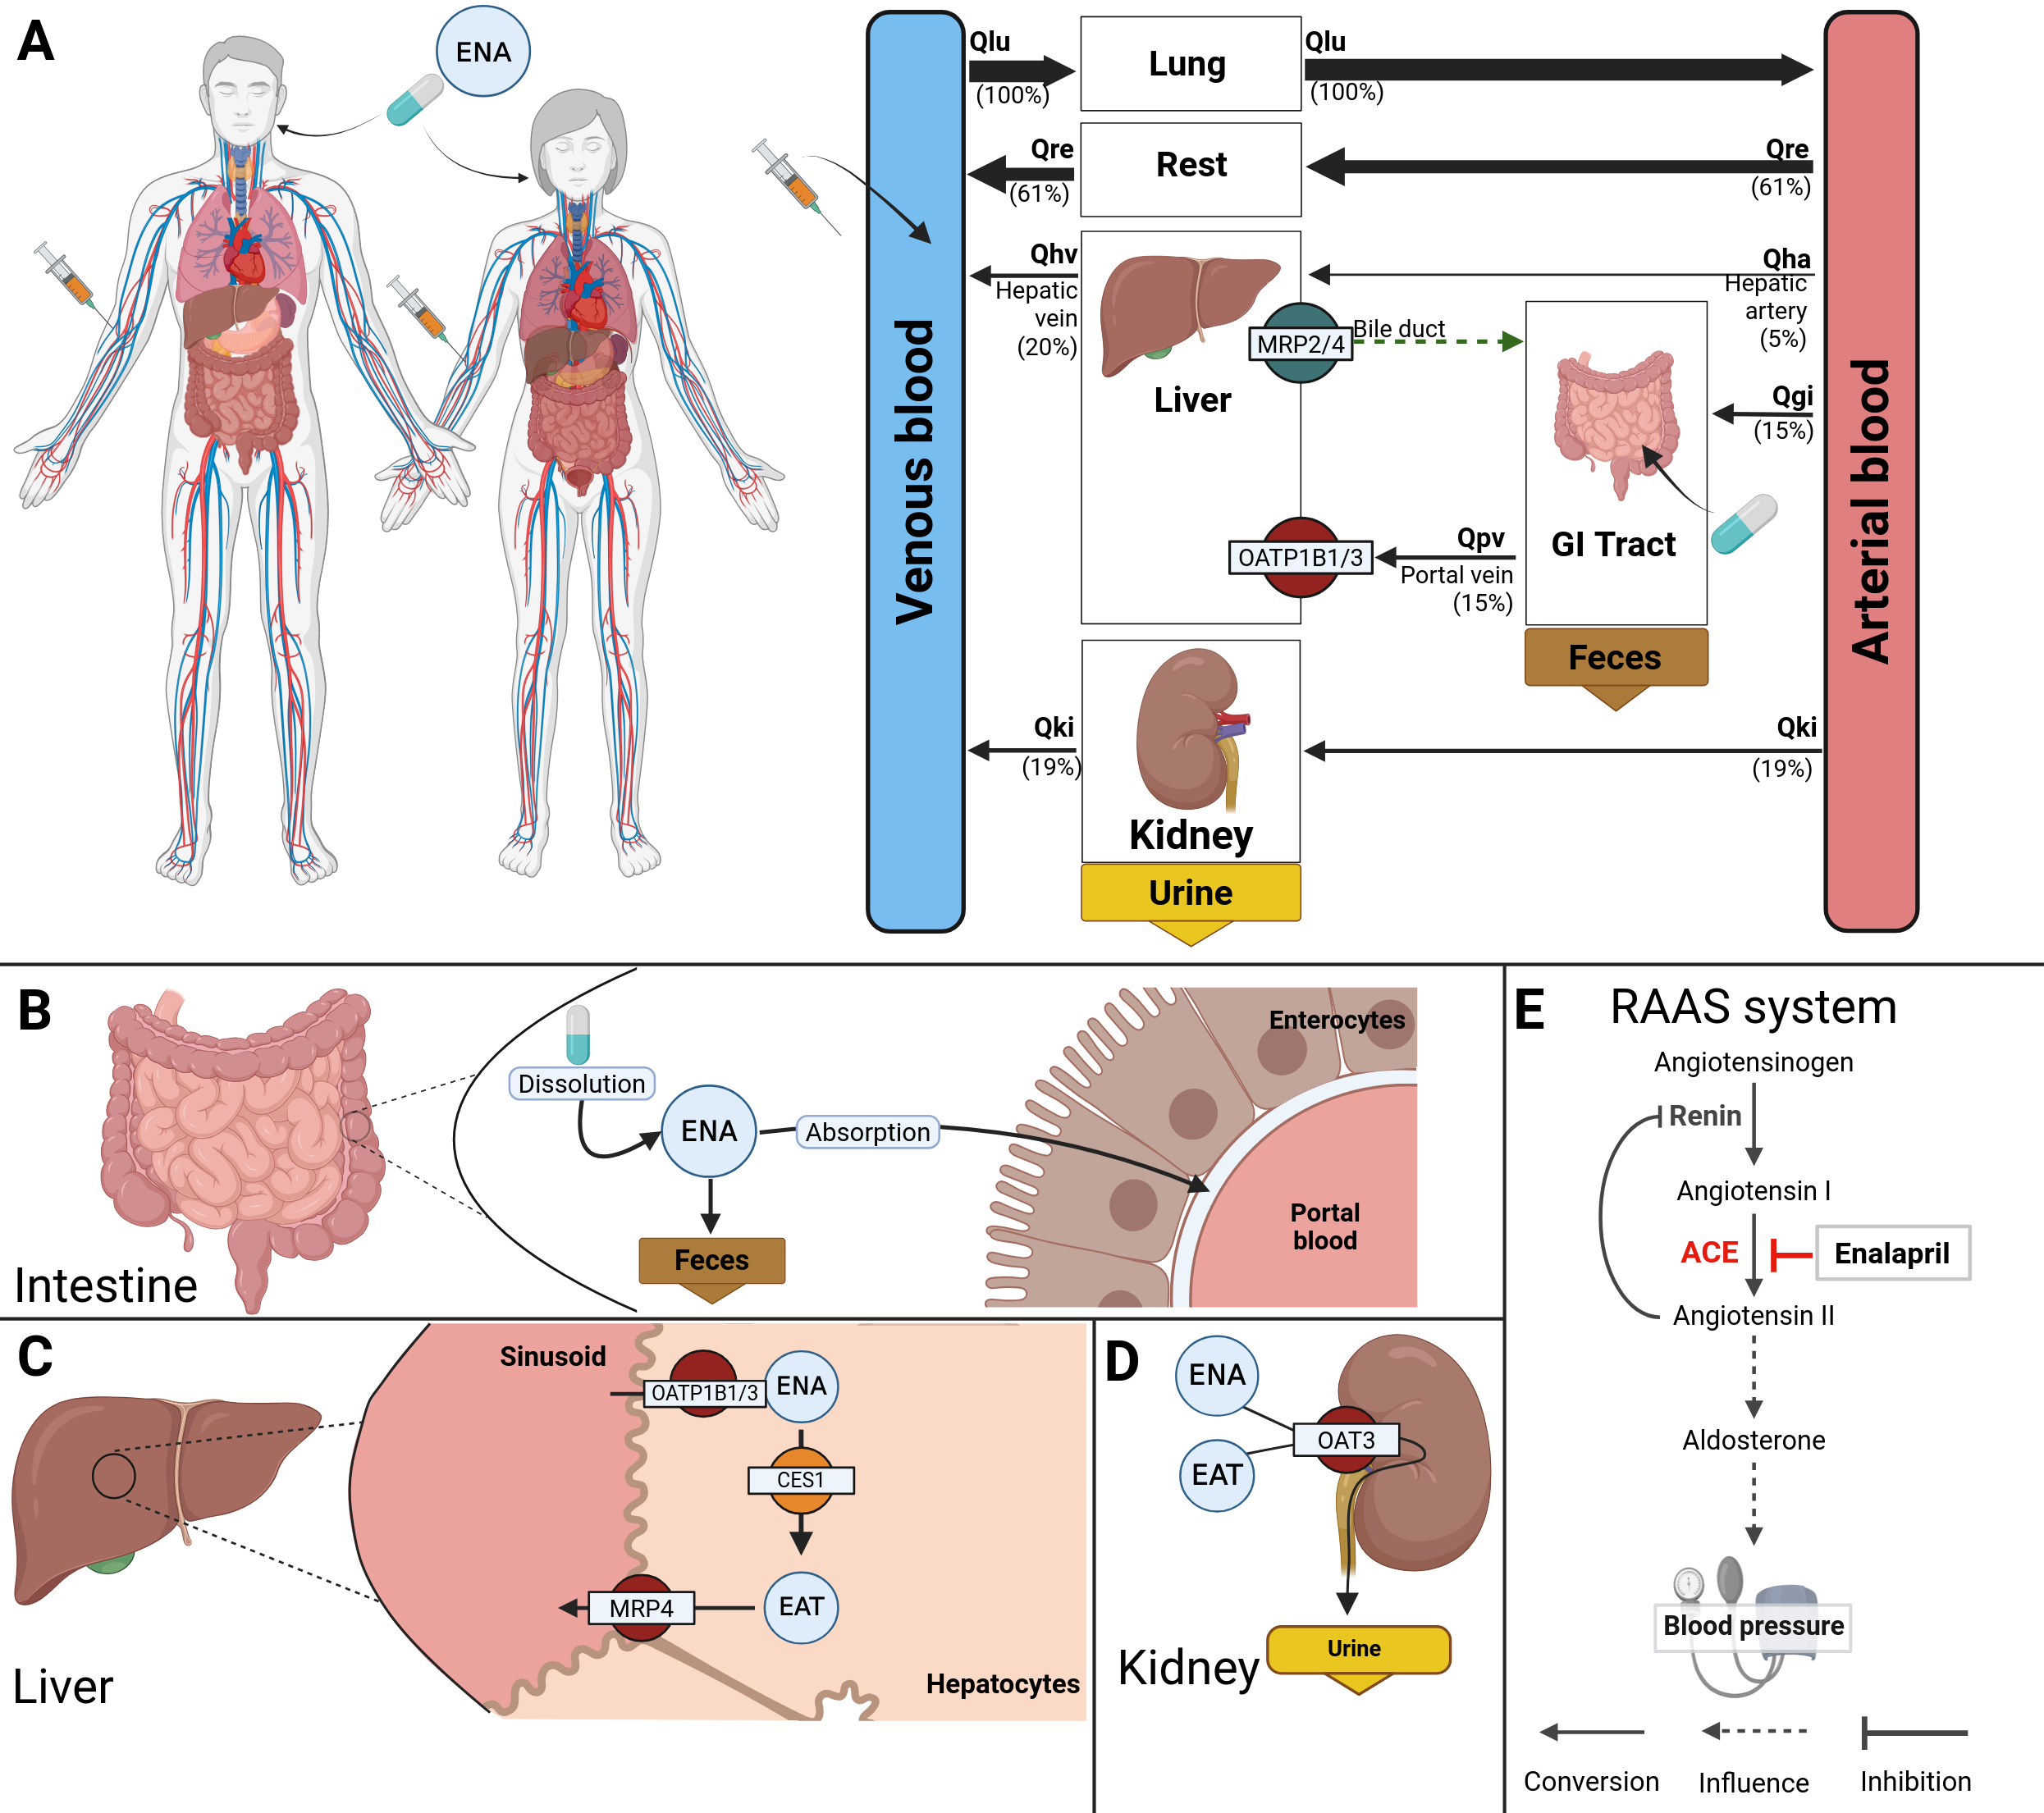
\includegraphics[width=0.99\linewidth]{figures/enalapril_model.png}
    \caption[PBPK model of enalapril]{\textbf{Overview of the physiologically-based model of enalapril.}} \textbf{(A)}~Whole body model showing cardio-pulomonary circulation via the blood. \textbf{(B)}~Intestine model showing dissolution and absorption of enalapril by enterocytes. \textbf{(C)}~Liver model with the uptake of enalapril by hepatocytes and its conversion to enalaprilat. \textbf{(D)}~Kidney model showing transport of enalapril and enalaprilat into the kidney and their subsequent excretion via urine. \textbf{(E)}~Schematic of the renin-angiotensin-aldosterone system (RAAS)  and the interfering/inhibitory role of enalapril
    \label{fig:enalapril_model}
\end{figure}

The PBPK model developed consists of a whole-body model linking different organs via the systemic circulation (Fig.~\ref{fig:enalapril_model}). The PBPK model follows a hierarchical structure, with the whole-body model linking sub-models for the intestine, kidney and liver.The model describes the metabolic and biochemical pathways in the tissue consisting of the transport of enalapril through the intestine, liver and kidney. Transport processes and biochemical reactions were modelled using reversible and irreversible Michaelis-Menten equations.

Liver impairment was modeled by scaling liver function with \texttt{f\_cirrhosis} from 0.0 (no cirrhosis) to 0.95 (critical cirrhosis), based on an indocyanine green model~\cite{Koller2021, Koller2021a} mapping CPT classes A, B, and C to parameter values of 0.40, 0.70, and 0.81, respectively. The Child-Turcotte-Pugh (CTP) score estimates mortality risk in cirrhotic patients using criteria originally outlined by Child and Turcotte~\cite{Child1964} and later modified by Pugh~\cite{Pugh1973}. Mechanistically, cirrhosis is represented by reduced functional liver volume alongside portosystemic blood shunting, both decreasing effective liver blood flow. 
Renal impairment was modeled as a progressive functional decline by scaling all renal processes with \texttt{f\_renal\_function} (1.0 = normal, 0.0 = none), applying KDIGO-based cut-offs~\cite{Stevens2024} for mild (0.69), moderate (0.32), and severe (0.19) stages~\cite{Mallol2023}.
Cardiac impairment was simulated by reducing total blood flow by 30\% using \texttt{f\_cardiac\_output} = 0.70.
Variations in CES1 activity were modeled by scaling the metabolic rate via \texttt{f\_ces1} (wild type = 1.0, $>1.0$ = increased, $<1.0$ = reduced). Modeled alleles included wild type (1.0), G143E (0.1), active allele (1.2), and CES1A1C (1.0), with overall function calculated as the average of both alleles (e.g., WT/G143E = 0.55).

% \subsection{Model Assumptions}
% \label{sec:methods_assumptions}

\subsection{Parameter optimization}
\label{sec:methods_fitting}
Parameter fitting was used to minimise the distance between experimental data and model predictions by optimising a subset of ten parameters of the model. For this purpose, a subset of curated time curves from healthy and hypertensive subjects after single dose application was used, as listed in Tab.
% ~\ref{tab:study_table}
Parameters were optimised in a multistep process based on the route of administration. First, parameters relevant to intravenous enalaprilat were optimised using the subset of intravenous data. Next, parameters for oral enalapril were optimised using a subset of the oral enalapril data. Finally, metabolic conversion and liver transport parameters were optimised. This strategy allowed the parameters of enalaprilat and enalapril to be determined separately with subsequent optimisation of the coupling step.

The cost function, which depends on the parameter $\vec{p}$, minimised the sum of the quadratic weighted residuals $r_{i,k}$ for all time courses $k$ and data points $i$. Time courses were weighted by the number of participants in each study $n_k$ and individual time points with the standard deviation $\sigma_{i,k}$ associated with the measurement, resulting in weights $w_{i,k} = n_k/\sigma_{i,k}$.

\begin{equation*}
   F(\vec{p})= 0.5 \sum_{i,k} (w_{i,k} \cdot r_{i,k}(\vec{p}))^2
\end{equation*}

Multiple optimisation runs (n=100) were performed with different initial parameters based on a local optimiser, with the optimal parameters used in the final model. The fitted parameters are shown in Tab.~\ref{tab:Parameter_Fitting}. For validation, all data after multiple applications, disease states, CES1 activity other than wild-type were used.

\subsection{Simulations}
\label{sec:methods_simulations}
For all curated clinical trials (Tab.~\ref{tab:study_table}), \textit{in silico} simulation experiments were created. For the simulations, the parameters corresponding to the the genetic variants (\texttt{f\_ces1}), pathophysiology (\texttt{f\_renal\_function}, \texttt{f\_cirrhos
is}, \texttt{f\_cardiac\_output}),  and the dosing (\texttt{PODOSE\_ena}, \texttt{IVDOSE\_ena}, \texttt{PODOSE\_eat}, \texttt{IVDOSE\_eat}) were modified according to the study. In the case of multiple dosing, the appropriate doses were given at the specified times. The model was then used to simulate the time courses of enalapril and enalaprilat in plasma and urine, and clinical data were compared with the model predictions.

\subsection{Parameter scans}
\label{sec:methods_scans}
Parameter scans were performed for a single oral dose of enalapril of 20~mg across three main cases: liver impairment, kidney impairment and CES1 gene activity. The parameters were scanned in the following ranges: \texttt{f\_cirrhosis} in linspace (0, 0.9, num=19) with normal liver function corresponding to 0.0; \texttt{f\_renal\_function} in logspace (-1, 1, num=19) with normal kidney function corresponding to 1.0; \texttt{f\_ces1} in logspace (-1, 1, num=19) with normal CES1 function corresponding to 1.0. 

\subsection{Pharmacokinetic and pharmacodynamic parameters}
\label{sec:methods_pkpd_parameters}
Pharmacokinetic parameters of enalapril and enalaprilat were calculated from plasma concentration time curves and urinary excretion using standard non-compartmental methods. The elimination rate $k\textsubscript{el}$[1/min] was calculated by linear regression in logarithmic space in the decay phase. The area under the curve AUC [mmole$\cdot$min/L] was calculated using the trapezoidal rule and extrapolated to infinity by linear interpolation. Apparent clearance $Cl$ [ml/min] was calculated as $Cl/F = k_\mathrm{el} \cdot V_\mathrm{d}$ with apparent volume of distribution $V_\mathrm{d}/F = D/(AUC_\infty \cdot k_{el})$. $D$ is the applied dose of enalapril maleate.
***pharmacodynamic parameters***